\label{sec:desc_env_all}
W poprzednim rozdziale omówiono sposoby implementacji w opracowanym oprogramowaniu VMC rozwiązania problemów stawianych przez tezę pracy (Rozdział \ref{sec:zakres-i-teza-pracy}). Zostały w nim przedstawione również wykorzystane nowoczesne technologie, takie jak konteneryzacja (Rozdział \ref{sec:docker}) oraz systemy do zarządzania kontenerami w środowisku chmurowym (Rozdział \ref{sec:k8s}), które dzięki zastosowaniu mechanizmu opisanego w rozdziale \ref{sec:scaling} pozwalają na optymalizacje obliczeń dla dużej ilości danych.

\bigbreak
W tym rozdziale przedstawiono opis trzech niezależnych, rzeczywistych środowisk teleinformatycznych, wykorzystanych do analiz umożliwiających weryfikacje poprawności założonej tezy (Rozdział \ref{sec:zakres-i-teza-pracy}). 
Opisy dotyczą podstawowych, ilościowych wyników związanych z liczbą wykrytych podatności przez oprogramowanie skanujące. Wykorzystane środowiska teleinformatyczne A, B i C są środowiskami rzeczywistymi, dlatego wszystkie adresy IP zostały zanimizowane. Dla środowiska teleinformatycznego A oprócz otrzymania raportów z wykrytymi podatnościami za pomocą oprogramowania Nessus \cite{beale2004nessus} otrzymano informacje na temat ustawień parametrów środowiskowych $CIA$, które szerzej opisane zostały w rozdziale \ref{sec:cia_desc}. Dla środowiska teleinformatycznego B otrzymano tylko raport z wykrytymi podatnościami za pomocą oprogramowania Nessus. Dla środowiska teleinformatycznego C otrzymano raport z wykrytymi podatnościami za pomocą oprogramowania Nessus oraz ogólne informacje dotyczące wag skanowanych zasobów. Niniejszy rozdział podzielony jest na pięć podrozdziałów. Pierwsze trzy podrozdziały poświęcone są opisom danych pochodzących ze środowisk teleinformatycznych. W czwartym podrozdziale przedstawiona została konfiguracja sprzętu oraz oprogramowania wykorzystana do zbadania modeli zarządzania podatnościami (Rozdział \ref{sec:modele-zarzadzaia-podatnosciami}), ponieważ właściciele zasobów udostępniający informacje na temat swoich środowisk teleinformatycznych nie wyrazili zgody na przetwarzanie danych w środowisku chmurowym. W ostatnim, piątym podrozdziale omówiono konfiguracje środowiska wykorzystaną do zbadana przyrastającej ilości danych na parametr $T_{VMC}$ (Rozdział \ref{sec:modele-ewaluacji-efektywnosci}), który jest miernikiem skuteczności działania rozwiązań przedstawionych w rozdziałach \ref{sec:docker}, \ref{sec:k8s}, \ref{sec:scaling}.

\section{Opis badanego środowiska teleinformatycznego A}
\label{sec:desc_a}
W środowisku teleinformatycznym A dostępne są 23 serwery odpowiadające za dostarczanie usług, takich jak portale internetowe dla wewnętrznych potrzeb organizacji, zawierające 36 podatności wykrytych przez skaner Nessus. Dodatkowo skaner zgłosił 322 podatności o kategorii informacyjnej, które zawierają w znacznej większości informacje na temat konfiguracji samego procesu skanowania oraz wykrytych otwartych portów i usług. Skan został wykonany bez autoryzacji, to znaczy bez logowania na skanowane zasoby. Skan został przeprowadzony w dniu 11.02.2021 i trwał 3 godziny.

\bigbreak
Tabela \ref{tab:chapter5:env_a:detected_vulns_nessus} przedstawia dokładną liczbę wykrytych podatności przez skaner Nessus z rozróżnieniem na oba standardy. Różnica pomiędzy liczbą wskazywaną przez raport Nessus a liczbą podatności według CVSS wynika z grupowania przez oprogramowanie skanujące niektórych CVE do jednej kategorii, przykładowo ujęta w raporcie podatność “134944 - PHP 7.3.x < 7.3.16 Multiple Vulnerabilities” posiada przypisane trzy CVE, mianowicie CVE-2020-7064, CVE-2020-7065, CVE-2020-7066. Różnica pomiędzy liczbą otrzymanych ocen bazowych CVSS 2.0 oraz CVSS 3.x wynika z problemu braku oceny dla tej samej podatności według obu standardów. Problem opisany został szerzej w rozdziale \ref{sec:modele-zarzadzaia-podatnosciami}.

\begin{table}[tbh]
\caption{Liczba wykrytych podatności według oceny bazowej CVSS dla środowiska A.}
\begin{center}
\label{tab:chapter5:env_a:detected_vulns_nessus}
\begin{tabular}{ccc}
\hline \noalign {\smallskip}
 & ocena bazowa CVSS 2.0 & ocena bazowa CVSS 3.x \\
\hline \noalign {\smallskip}
\textbf{Liczba Podatności}  &  41    & 27 \\
\hline \noalign {\smallskip}
\end{tabular}
\end{center}
\end{table}

\bigbreak
Rysunek \ref{fig:chapter5:env_a:env_stats} przedstawia histogram podziału kategorii podatności według ocen bazowych CVSS 2.0 oraz 3.x z której wynika, że znacząca większość wykrytych podatności, bo aż 83\% dla CVSS 2.0 oraz 52\% dla CVSS 3.x, są podatnościami o kategorii średniej (Rozdział \ref{sec:cvss_2_standard}, \ref{sec:cvss_3_standard}). Dokładna analiza wyników skanowania, podział kategorii oraz szacowana liczba roboczogodzin została przedstawiona w rozdziale czwartym.

\begin{figure}[!ht]
\centering
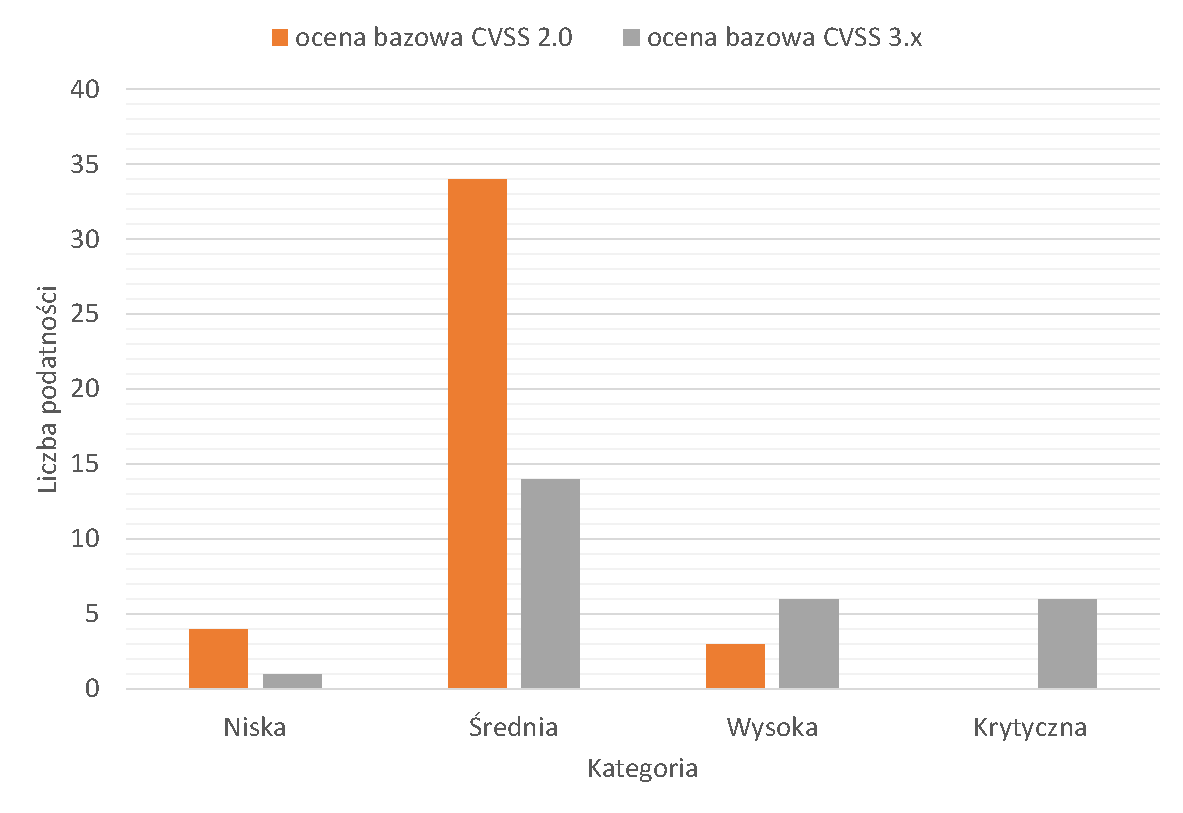
\includegraphics[width=.8\textwidth]{Chapters/Srodowiska/env_A/env_a_stats.pdf}
\caption{Histogram kategorii podatności z podziałem na oceny bazowe CVSS 2.0 i 3.x dla środowiska A.}
\label{fig:chapter5:env_a:env_stats}
\end{figure}


\bigbreak
Tabela \ref{tab:chapter5:env_a:cia} przedstawia rozkład parametrów środowiskowych $CIA$, który został dostarczony przez administratorów środowiska teleinformatycznego A. Dotyczy 5 skanowanych serwerów, co odpowiada 21.47\% wszystkich zasobów w testowanym środowisku. W związku z tym parametry $CIA$ ustawione są jako niezdefiniowane dla pozostałych 78.26\% serwerów. Parametr dotyczący wymagań dostępności (ang. Availability) ustawiony jest jako: wysoki dla 3 elementów sieci; średni dla 2 elementów sieci; co odpowiada 13.04\% i 8.7\%. Parametr dotyczący wymagań integralności (ang. Integrity) ustawiony jest jako: wysoki dla 1 serwera; średni dla 1 serwera, co odpowiada 4.35\%.

\begin{table}[tbh]
\caption{Rozkład parametrów $CIA$ dla środowiska A.}
\begin{center}
\label{tab:chapter5:env_a:cia}
\begin{tabular}{lllll}
\hline \noalign {\smallskip}
\textbf{Nazwa}           & Niska   & Średnia & Wysoka & Niezdefiniowana   \\
\hline \noalign {\smallskip}
\textbf{Poufność} &   13.04\%  &  4.35\%    & 4.35\%      &   78.26\% \\
\textbf{Integralność}       &   13.04\%  &  4.35\%    & 4.35\%      &   78.26\%  \\
\textbf{Dostępność}    &       0\%  &   8.7\%   & 13.04\%      &   78.26\%  \\
\hline \noalign {\smallskip}
\end{tabular}
\end{center}
\end{table}

%%%%%%%%%%%%%%%%%%%%%%%%%%%%%%%%%%%%%%%%%%%%%%%%

%%%%%%%%%%%%%%%%%%%%%%%%%%%%%%%%%%%%%%%%%%%%%%%%
\section{Opis badanego środowiska teleinformatycznego B}
\label{sec:desc_b}
W środowisku teleinformatycznym B dostępne jest 36 serwerów z różnymi niesprecyzowanym usługami, świadczonymi dla pracowników organizacji. Informacje o usługach uruchomionych na wskazanych serwerach są nieistotne z punktu widzenia przeprowadzonych analiz, które opisane zostały w rozdziale czwartym oraz piątym. Środowisko teleinformatyczne B zawiera 85 podatności wykrytych przez skaner Nessus. Dodatkowo skaner zgłosił 615 podatności o kategorii informacyjnej, które zawierają w znacznej większości informacje na temat konfiguracji samego procesu skanowania oraz wykrytych otwartych portów i usług. Skan został przeprowadzony w dniach od 04.05.2021 do 05.05.2021 i trwał 19 godzin.

\bigbreak
Tabela \ref{tab:chapter5:env_b:detected_vulns_nessus} przedstawia liczbę podatności wykrytych przez skaner Nessus z rozróżnieniem na oba standardy. Tak samo jak w przypadku środowiska teleinformatycznego A, różnica pomiędzy liczbą wskazywaną przez raport Nessus a liczbą podatności według oceny bazowej CVSS wynika z grupowania podatności przez oprogramowanie skanujące niektórych CVE do jednej kategorii. Różnica pomiędzy liczbą CVSS 2.0 oraz CVSS 3.x wynika z problemu braku oceny bazowej dla tej samej podatności według obu standardów. Problem opisany został szerzej w rozdziale \ref{sec:modele-zarzadzaia-podatnosciami}.

\begin{table}[tbh]
\caption{Liczba wykrytych podatności według oceny bazowej CVSS dla środowiska B.}
\begin{center}
\label{tab:chapter5:env_b:detected_vulns_nessus}
\begin{tabular}{ccc}
\hline \noalign {\smallskip}
                &  ocena bazowa CVSS 2.0 & ocena bazowa CVSS 3.x\\
\hline \noalign {\smallskip}
\textbf{Liczba Podatności} &      104       & 54    \\
\hline \noalign {\smallskip}
\end{tabular}
\end{center}
\end{table}

\bigbreak
Rysunek \ref{fig:chapter5:env_a:env_stats} przedstawia histogram podziału kategorii podatności według oceny bazowej CVSS 2.0 oraz 3.x, z której wynika, że znacząca większość wykrytych podatności, bo aż 90\% dla CVSS 2.0 oraz 55\% dla CVSS 3.x, są podatnościami o kategorii średniej (Rozdział \ref{sec:cvss_2_standard}, \ref{sec:cvss_3_standard}). Dokładne omówienie wyników skanowania, podział kategorii oraz szacowana liczba roboczogodzin zostaną przedstawione w rozdziale czwartym.

\bigbreak
Dla środowiska teleinformatycznego B, administrator nie dostarczył żadnych informacji, z których możliwe byłoby określenie wartości parametrów środowiskowych $CIA$ (Rozdział \ref{sec:cia_desc}), w związku z czym wytworzone oprogramowanie VMC na potrzeby przeprowadzonych analiz dla wszystkich wartości parametrów przyjęto wartość niezdefiniowaną, która jak opisano w rozdziale \ref{sec:cia_desc}, nie ma wpływu na otrzymaną ocenę środowiskową. 

\begin{figure}[!ht]
\centering
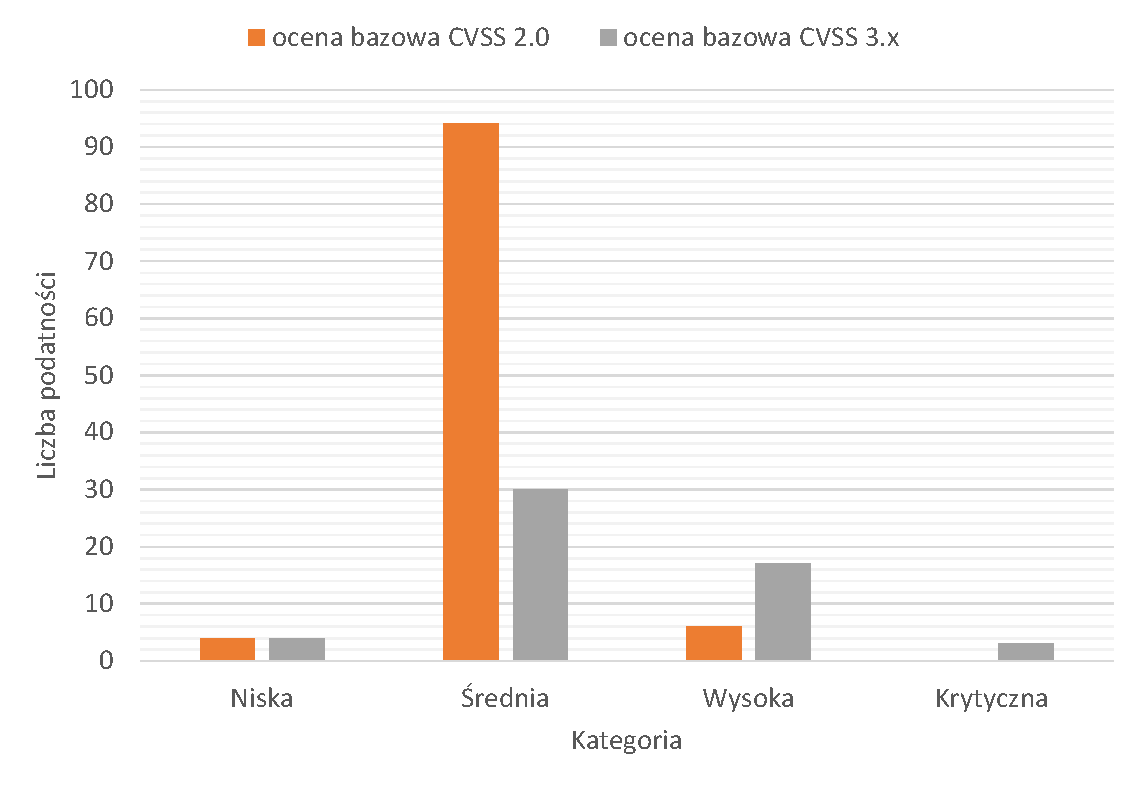
\includegraphics[width=.8\textwidth]{Chapters/Srodowiska/env_B/env_b_stats.pdf}
\caption{Histogram kategorii podatności z podziałem na ocenę bazową CVSS 2.0 i 3.x dla środowiska B.}
\label{fig:chapter5:env_b:env_stats}
\end{figure}



%%%%%%%%%%%%%%%%%%%%%%%%%%%%%%%%%%%%%%%%%%%%%%%%

%%%%%%%%%%%%%%%%%%%%%%%%%%%%%%%%%%%%%%%%%%%%%%%%
\section{Opis badanego środowiska teleinformatycznego C}
\label{sec:desc_c}
W środowisku teleinformatycznym C dostępne są 2 062 urządzenia sieciowe, czyli cała wewnętrzna infrastruktura organizacji, dla której skaner Nessus wykrył 2 949 podatności. Dodatkowo skaner zgłosił 16 640 podatności o kategorii informacyjnej, które zawierają w znacznej większości informacje na temat konfiguracji samego procesu skanowania oraz wykrytych otwartych portów i usług. Skan został częściowo wykonany z autoryzacją, mianowicie skaner posiadał możliwość zalogowania się na 41 urządzeniach sieciowych, co stanowi niecałe 2\% badanego środowiska. Skan został przeprowadzony w dniach od 26.04.2021 do 27.04.2021 i trwał 23 godziny. 

\bigbreak
Tabela \ref{tab:chapter5:env_c:detected_vulns_nessus} przedstawia liczbę podatności wykrytych przez skaner Nessus z rozróżnieniem na oba standardy. Tak samo jak w przypadku środowiska teleinformatycznego A i B, różnica pomiędzy liczbą wskazywaną przez raport Nessus a liczbą podatności według oceny bazowej CVSS wynika z tego, że Nessus grupuje niektóre CVE do jednej kategorii. Różnica pomiędzy liczbą ocen bazowych CVSS 2.0 oraz CVSS 3.x wynika z problemu braku oceny dla tej samej podatności według obu standardów. Problem opisany szerzej został w rozdziale \ref{sec:modele-zarzadzaia-podatnosciami}.

\begin{table}[tbh]
\caption{Liczba wykrytych podatności według oceny bazowe CVSS dla środowiska C.}
\begin{center}
\label{tab:chapter5:env_c:detected_vulns_nessus}
\begin{tabular}{ccc}
\hline \noalign {\smallskip}
   & ocena bazowa CVSS 2.0 & ocena bazowa CVSS 3.x \\
\hline \noalign {\smallskip}
\textbf{Liczba Podatności}   &      10 078 &         9 730 \\
\hline \noalign {\smallskip}
\end{tabular}
\end{center}
\end{table}

\bigbreak
Rysunek \ref{fig:chapter5:env_c:env_stats} przedstawia histogram kategorii podatności według ocen bazowych CVSS 2.0 oraz CVSS 3.x. Na podstawie wyników z rysunku \ref{fig:chapter5:env_c:env_stats} można stwierdzić, że znacząca większość wykrytych podatności, bo aż 65\% dla CVSS 2.0 oraz 46\% dla CVSS 3.x, są podatnościami o kategorii średniej (Rozdział \ref{sec:cvss_2_standard}, \ref{sec:cvss_3_standard}).


\begin{figure}[!ht]
\centering
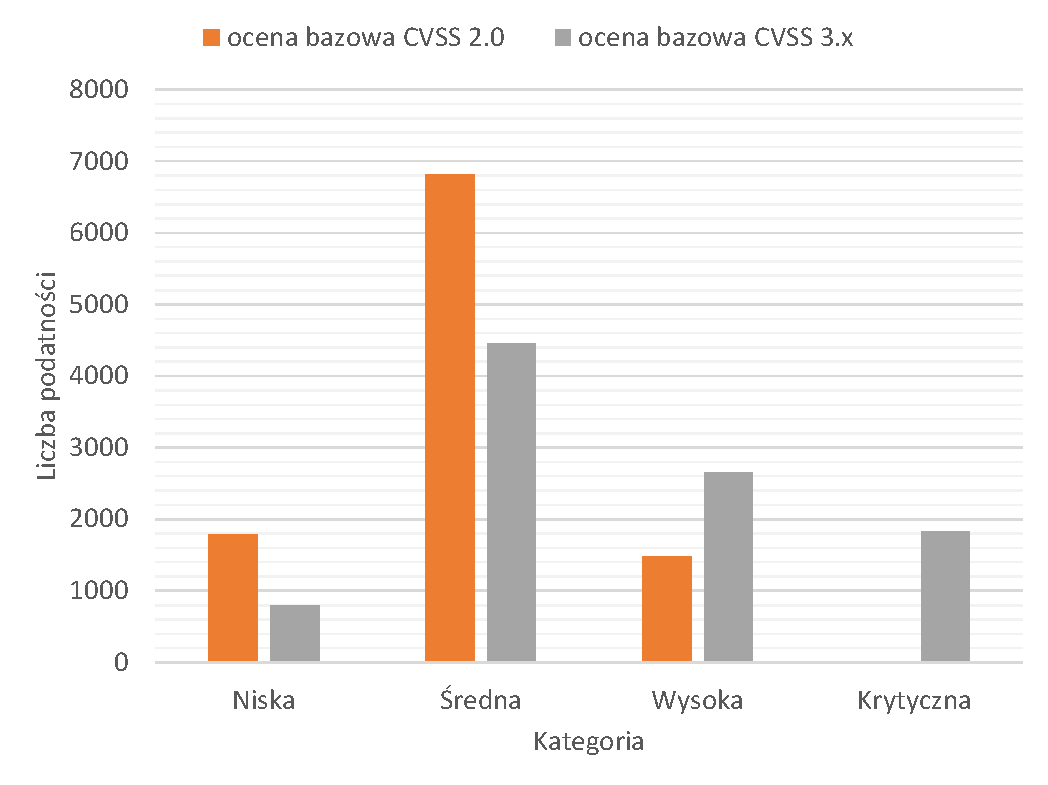
\includegraphics[width=.7\textwidth]{Chapters/Srodowiska/env_C/env_c_stats.pdf}
\caption{Histogram kategorii podatności z podziałem na oceny bazowe CVSS 2.0 i 3.x dla środowiska C.}
\label{fig:chapter5:env_c:env_stats}
\end{figure}


\bigbreak
Dla środowiska teleinformatycznego C administrator dostarczył tylko ogólne informacje dotyczące wagi skanowanych zasobów (podział: niskie, średnie, krytyczne), z których wynika, że 217 urządzeń określonych jest wagą krytyczną, 790 oznaczonych wagą średnią, 851 wagą niską z punktu widzenia organizacji. Dla 204 zasobów administrator nie dostarczył żadnych informacji. Całościowy rozkład wag zasobów przedstawiony został na rysunku \ref{fig:chapter5:env_c:os_cia}.

\begin{figure}[!ht]
\centering
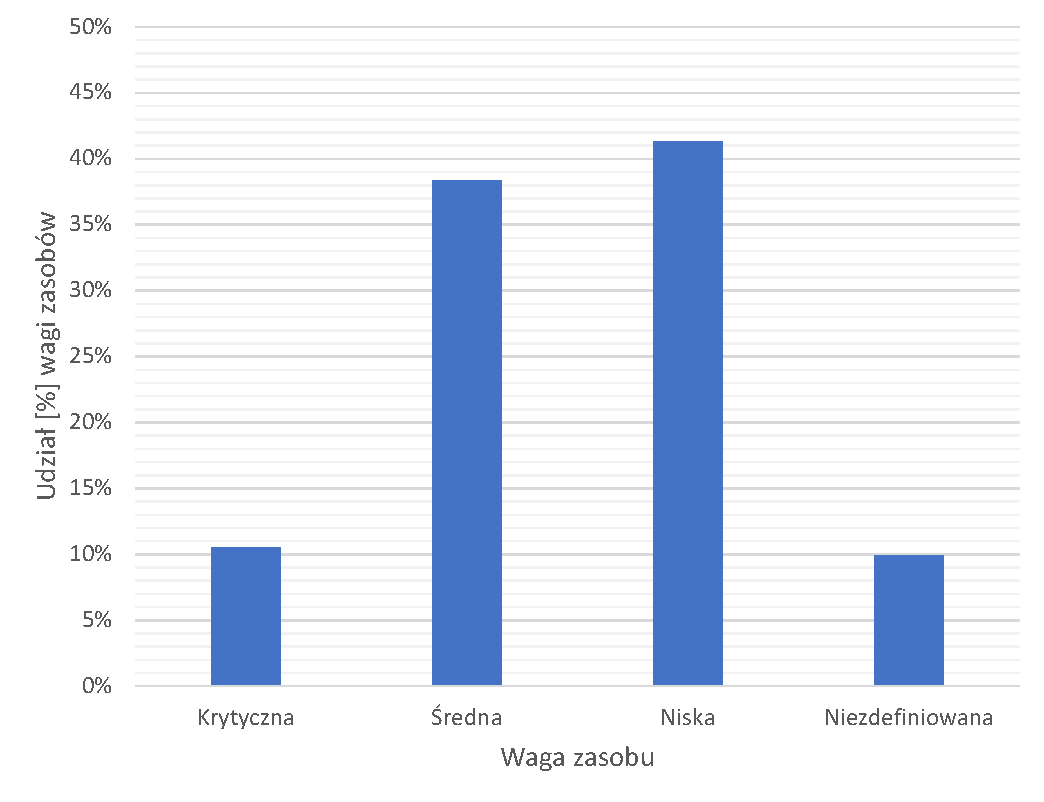
\includegraphics[width=.7\textwidth]{Chapters/Srodowiska/env_C/os_cia.pdf}
\caption{Histogram wag zasobów dla środowiska C.}
\label{fig:chapter5:env_c:os_cia}
\end{figure}

%%%%%%%%%%%%%%%%%%%%%%%%%%%%%%%%%%%%%%%%%%%%%%%%

%%%%%%%%%%%%%%%%%%%%%%%%%%%%%%%%%%%%%%%%%%%%%%%%
\section{Środowisko badawcze do pomiaru wpływu zmiany priorytetyzacji}
\label{sec:desc_pio}
Ponieważ organizacje, które udostępniły informacje na temat swoich środowisk teleinformatycznych (A, B, C) oraz wykrytymi w nich podatnościami za pomocą oprogramowania Nessus, nie wyraziły zgody na przetwarzanie danych w infrastrukturze zewnętrznej (w chmurze). W celu przeprowadzenia analiz potwierdzających tezę opisaną w rozdziale \ref{sec:zakres-i-teza-pracy}, zaimplementowane oprogramowanie na potrzeby pracy (Rozdział \ref{sec:vmc}) zostało uruchomione na komputerze MacBook Pro 2018 z procesorem 2.6 GHz Intel Core i7 oraz 32 GB 2400 MHz DDR4, wykorzystując technologię Docker (Rozdział \ref{sec:docker}) w następującej konfiguracji:
\begin{itemize}
\item Moduł obliczeniowy (ang. Processing Module) 
\item Monitor zdań (ang. Task monitor)
\item Panel Administratora (ang. Admin Panel)
\item Moduł pobierający informacje o zasobach infrastruktury teleinformatycznej (ang. Asset Collector)
\item Moduł pobierający informacje o wykrytych podatnościach w infrastrukturze teleinformatycznej (ang. Vulnerability Collector)
\item Baza danych PostgreSQL \cite{postgresql1996postgresql} - przechowywanie konfiguracji VMC 
\item Baza danych MariaDB \cite{bartholomew2012mariadb} - przechowywanie informacji o zasobach IT
\item Ralph \cite{ralph} - Panel administracyjny bazy zasobów IT 
\item Rabbitmq \cite{johansson2020rabbitmq} - system kolejkowy używany do komunikacji pomiędzy modułami VMC 
\item Baza Redis \cite{chen2016towards} - in-memory używana do przechowywania częściowych obliczeń i synchronizacji modułów VMC 
\item Elasticsearch  \cite{dixit2016elasticsearch} - baza tekstowa przechowująca informacje o wszystkich podatnościach 
\item Kibana \cite{gupta2015kibana} - graficzny interfejs pozwalający w łatwy sposób wyszukiwać wyniki oraz tworzyć metryki 
\end{itemize}

%%%%%%%%%%%%%%%%%%%%%%%%%%%%%%%%%%%%%%%%%%%%%%%%

%%%%%%%%%%%%%%%%%%%%%%%%%%%%%%%%%%%%%%%%%%%%%%%%
\section{Środowiska badawcze do analizy skalowalności rozwiązania}
\label{sec:desc_skalowalnosc}
W celu przeprowadzenia analiz dotyczących wpływu przyrastającej ilości przetwarzanych danych na parametr $T_{VMC}$ wprowadzonym w rozdziale \ref{sec:modele-ewaluacji-efektywnosci}. Zaimplementowane na potrzeby pracy oprogramowanie (\ref{sec:vmc}) zostało uruchomione w Microsoft Azure\textsuperscript{\textregistered} Free Tier subscription \cite{microsoft-fre-tier}. Ze względu na napotkane ograniczenia licencyjne, dotyczące możliwości wykorzystywania zasobów na bezpłatnej subskrypcji w jednym centrum danych, wykorzystano dwa niezależne centra danych: US West USA i US West USA 2, które w komunikacji między sobą wykazują średnie opóźnienie na poziomie 22 ms \cite{microsoft-latency}. W regionie US West 2 uruchomiono klaster kubernetes (\ref{sec:k8s}) składający się z 2 serwerów, każdy z procesorami 2$\times$ Intel Xeon\textsuperscript{\textregistered} E5-2673 v3 (Haswell) 2,4 GHz i 7 GB pamięci RAM z następującymi usługami:

\begin{itemize}
\item Moduł obliczeniowy (ang. Processing Module) 
\item Monitor zdań (ang. Task monitor)
\item Panel Administratora (ang. Admin Panel)
\item Moduł pobierający informacje o zasobach (ang. Asset Collector) 
\item Baza danych PostgreSQL \cite{postgresql1996postgresql} - przechowywanie konfiguracji VMC
\item Baza danych MariaDB \cite{bartholomew2012mariadb} - przechowywanie informacji o zasobach IT
\item Ralph \cite{ralph} - Panel administracyjny bazy zasobów IT
\item Rabbitmq \cite{johansson2020rabbitmq} - system kolejkowy używany do komunikacji pomiędzy modułami VMC
\item Baza Redis \cite{chen2016towards} - in-memory używana do przechowywania częściowych obliczeń i synchronizacji modułów VMC
\end{itemize}

\bigbreak
W regionie USA West został uruchomiony klaster Elasticsearch składający się z 2 serwerów, każdy o konfiguracji 1 $\times$ CPU Intel Xeon\textsuperscript{\textregistered} E5-2673 v3 (Haswell) 2,4 GHz, 3,5 GB pamięci RAM. Pomiędzy regionami utworzono sieć wirtualną (VLan).